\documentclass{article}


% if you need to pass options to natbib, use, e.g.:
%     \PassOptionsToPackage{numbers, compress}{natbib}
% before loading neurips_2023


% ready for submission
\usepackage[final]{neurips_2023}
\usepackage{graphicx}
\usepackage{array}
\usepackage{hyperref}
\usepackage{amsmath}
\usepackage{subfigure}
\usepackage{titlesec}
\titlespacing{\subsection}{0pt}{*1}{*1}

% to compile a preprint version, e.g., for submission to arXiv, add add the
% [preprint] option:
%     \usepackage[preprint]{neurips_2023}


% to compile a camera-ready version, add the [final] option, e.g.:
%     \usepackage[final]{neurips_2023}


% to avoid loading the natbib package, add option nonatbib:
%    \usepackage[nonatbib]{neurips_2023}


\usepackage[utf8]{inputenc} % allow utf-8 input
\usepackage[T1]{fontenc}    % use 8-bit T1 fonts
\usepackage{hyperref}       % hyperlinks
\usepackage{url}            % simple URL typesetting
\usepackage{booktabs}       % professional-quality tables
\usepackage{amsfonts}       % blackboard math symbols
\usepackage{nicefrac}       % compact symbols for 1/2, etc.
\usepackage{microtype}      % microtypography
\usepackage{xcolor}         % colors


\title{Neural Network for Fashion MNIST Dataset Using Low-Level Functions}


% The \author macro works with any number of authors. There are two commands
% used to separate the names and addresses of multiple authors: \And and \AND.
%
% Using \And between authors leaves it to LaTeX to determine where to break the
% lines. Using \AND forces a line break at that point. So, if LaTeX puts 3 of 4
% authors names on the first line, and the last on the second line, try using
% \AND instead of \And before the third author name.


\author{%
  Connor Gag \\
  \texttt{cgag@ucsd.edu} \\
  \And
  Shivangi Karwa \\
  \texttt{skarwa@ucsd.edu} \\
}



\begin{document}


\maketitle


\begin{abstract}
  This project focuses on developing a neural network to predict types of clothing in the Fashion MNIST dataset. We did this using various architectures and hyperparameters, without the use of popular machine learning libraries such as TensorFlow and PyTorch. The main package that we did use is NumPy, which is helpful for tasks such as calculations during backpropagation. Additionally, we added momentum and regularization and tested different activation functions. We experimented with hyperparameter tuning for regularization and found that L2 regularization converged in smoother way than L1 regularization, but their accuracies were about the same. In our experiments with activation functions, we found that ReLU performed better than Sigmoid. Overall, our best accuracy was about 88\% on the test data, which we achieved using momentum and regularization. 
\end{abstract}


\section{Data visualization}
We used the \href{https://www.kaggle.com/datasets/zalando-research/fashionmnist}{FashionMNIST Dataset}, which has different types of clothing.

\begin{figure}[h!tbp]
    \centering
    \begin{minipage}[t]{0.45\textwidth}
        \centering
        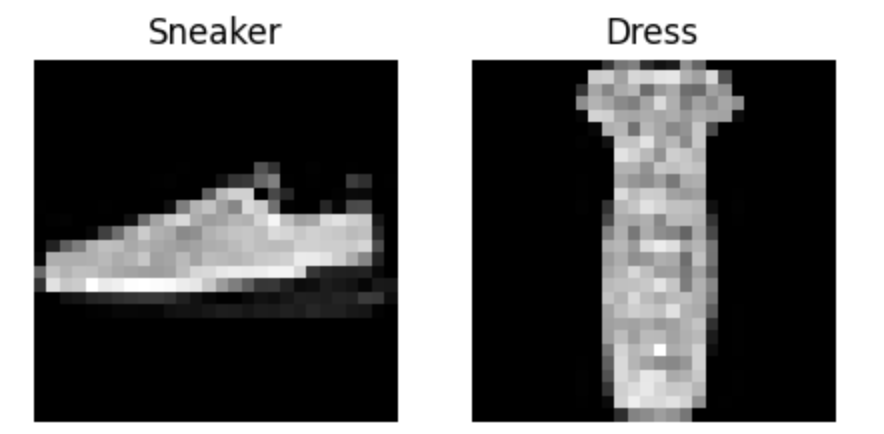
\includegraphics[width=\textwidth]{data_visualization.png}
        \caption{Data Visualization}
        \label{fig:data_visualization}
    \end{minipage}%
    \hspace{0.05\textwidth} % Adjust space between image and table
    \begin{minipage}[t]{0.45\textwidth}
        \centering
        \begin{tabular}{|>{\centering\arraybackslash}p{2cm}|>{\raggedright\arraybackslash}p{3cm}|}
            \hline
            \textbf{Data Label} & \textbf{Article of Clothing} \\ \hline
            0 & T-Shirt \\ \hline
            1 & Trouser \\ \hline
            2 & Pullover \\ \hline
            3 & Dress \\ \hline
            4 & Coat \\ \hline
            5 & Sandal \\ \hline
            6 & Shirt \\ \hline
            7 & Sneaker \\ \hline
            8 & Bag \\ \hline
            9 & Ankle Boot \\ \hline
        \end{tabular}
        \caption{Data Labels and Their Meanings}
        \label{table:data_labels}
    \end{minipage}
\end{figure}



\section{Data preprocessing}
The \href{https://www.kaggle.com/datasets/zalando-research/fashionmnist}{FashionMNIST Dataset}, consists of 70,000 28x28 images of different types of clothing. One training example consists of the 784 pixel values of an image.

We split the training data into a 80\%/20\% train/validation split.

\begin{table}[h!tbp]
\centering
\begin{tabular}{|c|c|}
\hline
\textbf{Data Set} & \textbf{Number of Examples} \\ \hline
Training Set & 48,000 \\ \hline
Validation Set & 12,000 \\ \hline
Test Set & 10,000 \\ \hline
\end{tabular}
\vspace{0.3cm}
\caption{Data Set Splits}
\label{table:data_splits}
\end{table}


We normalized the data by subtracting the mean of the whole image from each pixel, then dividing each pixel by the standard deviation.

\begin{table}[h!tbp]
\centering
\begin{tabular}{|>{\centering\arraybackslash}m{4cm}|>{\centering\arraybackslash}m{3cm}|>{\centering\arraybackslash}m{3cm}|}
\hline
\textbf{Statistic}           & \textbf{Before Normalization} & \textbf{After Normalization} \\ \hline
Mean                         & 0.26914766                & 9.73137e-09              \\ \hline
Standard Deviation (Std)     & 0.29125977                & 1.0                       \\ \hline
\end{tabular}
\vspace{0.3cm}
\caption{Comparison of Mean and Standard Deviation Before and After Normalization for One Image}
\label{table:normalization_stats}
\end{table}


\section{Softmax regression}
We trained the model using stochastic gradient descent. We added a softmax function as the output activation function in our last layer. This gave us the probabilities of our model's predictions:

$\sigma(a_j) = \frac{e^{a_j}}{\sum_{i=1}^{K} e^{a_i}}$

As for our architecture, we used two layers: an input layer (784 neurons) and an output layer (10 neurons). 

For our hyperparameters, our learning rate was .01 and changing the learning rate to .001 resulted in a slightly worse accuracy in the 100 epochs. Increasing the epochs would allow the model with this learning rate the time it needs to converge.


We set training to run for 100 epochs, but it stopped around 34 epochs because of our early stopping policy (3 epochs). Changing our early stopping policy to 5 epochs resulted in the model training for longer with no increase in accuracy.

We did not yet use regularization or momentum at this point. We used the config\_4.yaml. 




- The test accuracy is \textbf{84.15\%}.

- The test loss is 0.45745.


\begin{figure}[h!]
    \centering
    \subfigure[Accuracy]{
        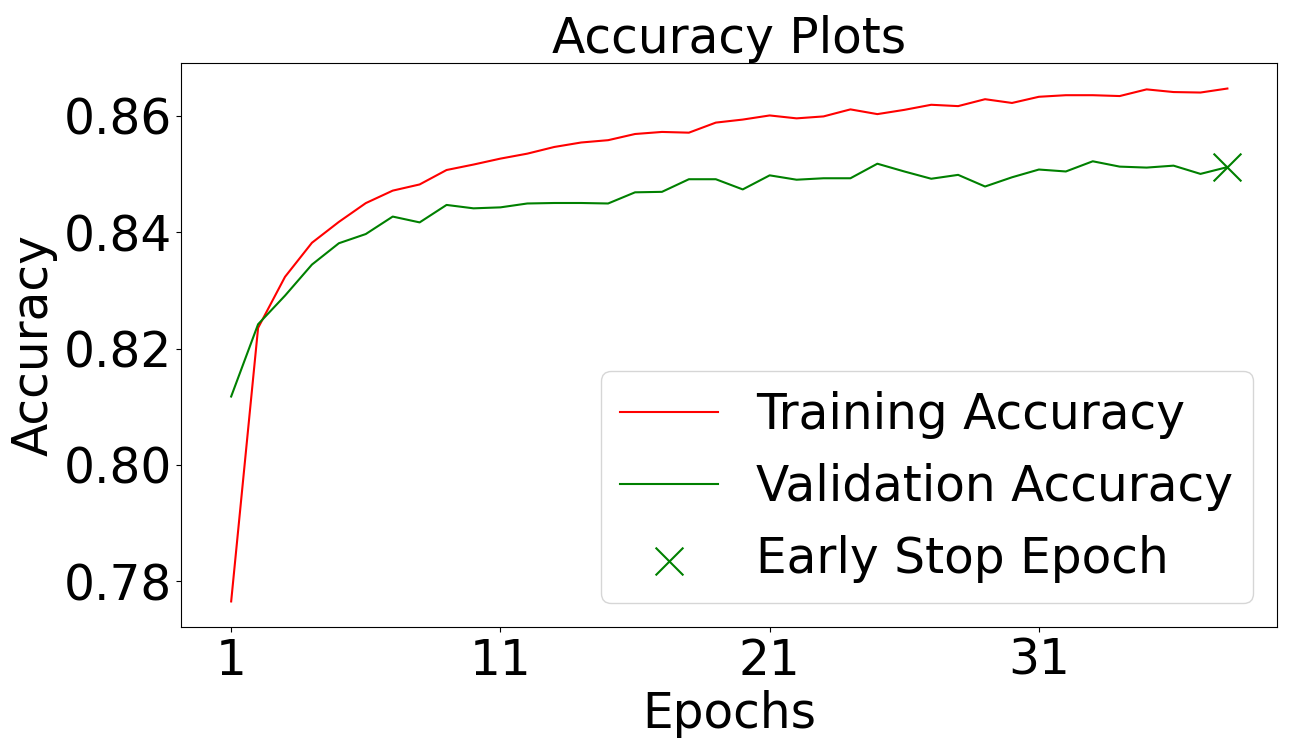
\includegraphics[width=0.45\textwidth]{accuracy_softmax.png}
        \label{fig:softmax_accuracy}
    }
    \hfill
    \subfigure[Loss]{
        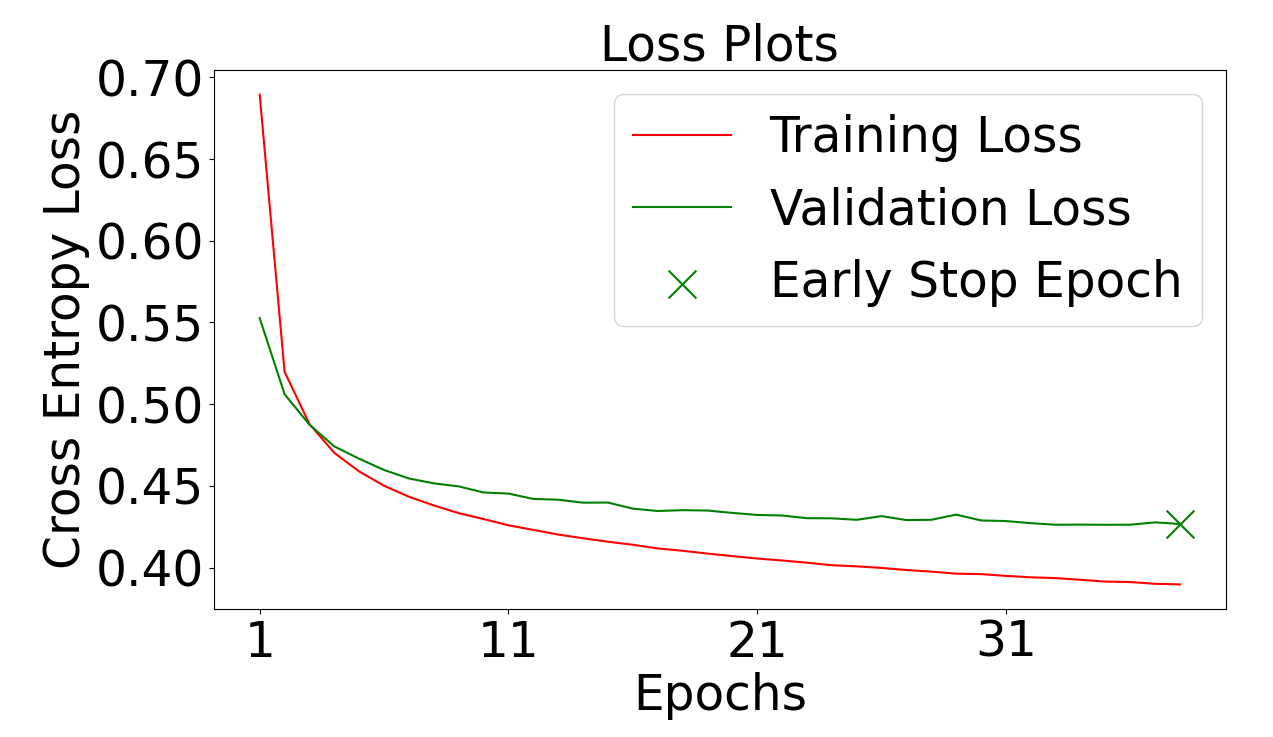
\includegraphics[width=0.45\textwidth]{cross_entropy_loss_softmax.png}
        \label{fig:softmax_loss}
    }
    \caption{Loss and Accuracy with Softmax}
    \label{fig:loss_acc_softmax}
\end{figure}



\section{Backpropagation}
To test our backpropagation, we implemented a gradient check. This manually computes the gradients by finding the difference in loss between small changes in a single random weight. This loss is then used to compute the gradient. 
This is the equation used: 
\[
\frac{d}{dw} E^n(w) \approx \frac{E^n(w + \epsilon) - E^n(w - \epsilon)}{2\epsilon}
\]

Epsilon = $10^{-2}$

We then compared this with the gradient computed with our backwards pass.

Architecture: 785 (+1 bias) $\rightarrow$ 128 (+1 bias) $\rightarrow$ 10 

These gradient tests were done with a trained model.


\begin{table}[hbt!]
\centering
\begin{tabular}{|p{3.8cm}|p{1.3cm}|p{2.1cm}|p{2.01cm}|p{2.1cm}|}
\hline
\textbf{Weight Type} & \textbf{Weight Index} & \textbf{Gradient (Backprop)} & \textbf{Gradient (Numerical)} & \textbf{Difference (Abs)} \\ \hline
Output Bias Weight   &           784, 79           &           1.831570e-13                   &         -2.775558e-13                      &         4.607127e-13             \\ \hline
Hidden Bias Weight   &            128, 1          &         0.001381                     &       0.001381                        &         2.291352e-08             \\ \hline
Hidden $\rightarrow$ Output Weight 1 &    304, 81   &      7.494840e-06                        &          3.170658e-06                     &             4.324181e-06         \\ \hline
Hidden $\rightarrow$ Output Weight 2 &   181, 40    &        -4.270080e-14                      &      -3.365363e-14                         &       9.047170e-15               \\ \hline
Input $\rightarrow$ Hidden Weight 1  &    44, 7   &        -5.081859e-07                       &                -5.081944e-07               &         8.461761e-12             \\ \hline
Input $\rightarrow$ Hidden Weight 2  &    47, 2   &        -7.732324e-09                      &            -7.732463e-09                   &        1.382703e-13              \\ \hline
\end{tabular}
\vspace{0.3cm}
\caption{Gradient verification for random weights.}
\label{tab:gradient_check}
\end{table}

\vspace{1cm}

\section{Momentum experiments}

We used the vectorized update rule and performed mini-batch gradient descent to train our classifier. The classifier was implemented with a neural network consisting of 128 hidden units and momentum integrated into the gradient descent process.
The hyperparameters were sourced from \textit{config\_6.yaml} file and detailed are as follows -

Learning rate - 0.001\\
Early stop epoch: 5\\
Momentum gamma - 0.9

The momentum was incorporated to the backward pass in our neural network model in the Layer class. The update rule for weights \( W \) with momentum is typically:
\[
v = \gamma v - \eta \nabla W
\]
\[
W = W + v
\]

where,
v is the velocity vector
$\gamma$ is the momentum
$\eta$ is the learning rate


To analyze the effectiveness of momentum, we conducted experiments using various learning rates and early stopping parameters. The best performance was achieved using the hyperparameters specified above. The final test accuracy of the model was:

Test Accuracy: \textbf{88.18\%}

Momentum helped accelerate convergence and provided more stable training compared to gradient descent without momentum. The early stopping mechanism helped prevent overfitting.

The following plots illustrate the model’s performance through the epochs - 
\begin{figure}[h!]
    \centering
    \subfigure[Loss]{
        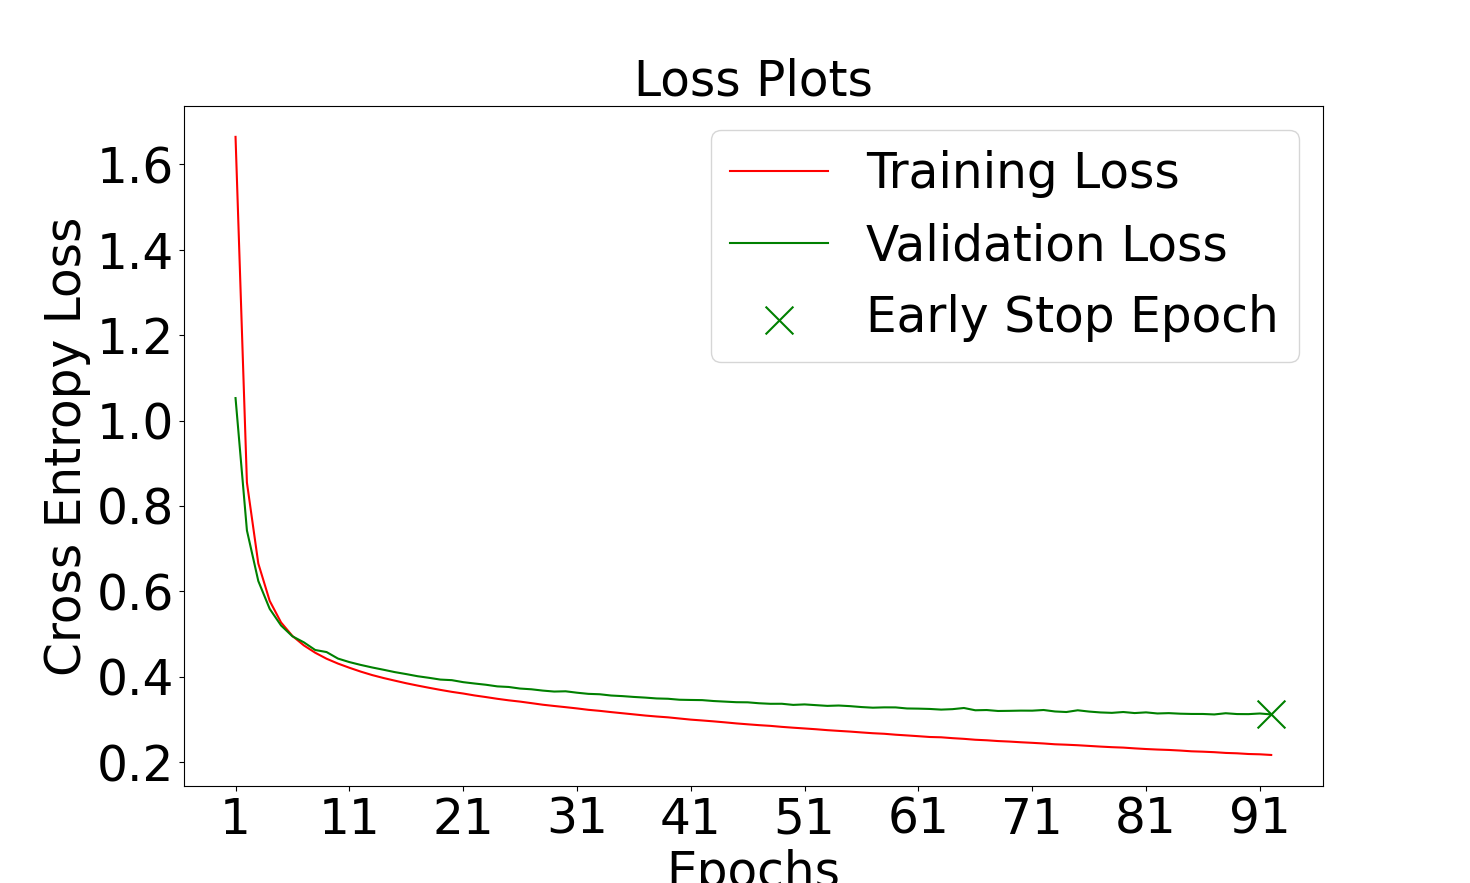
\includegraphics[width=0.45\textwidth]{Figure_mom.png}
        \label{fig:loss_lambda_1e4}
    }
    \hfill
    \subfigure[Accuracy]{
        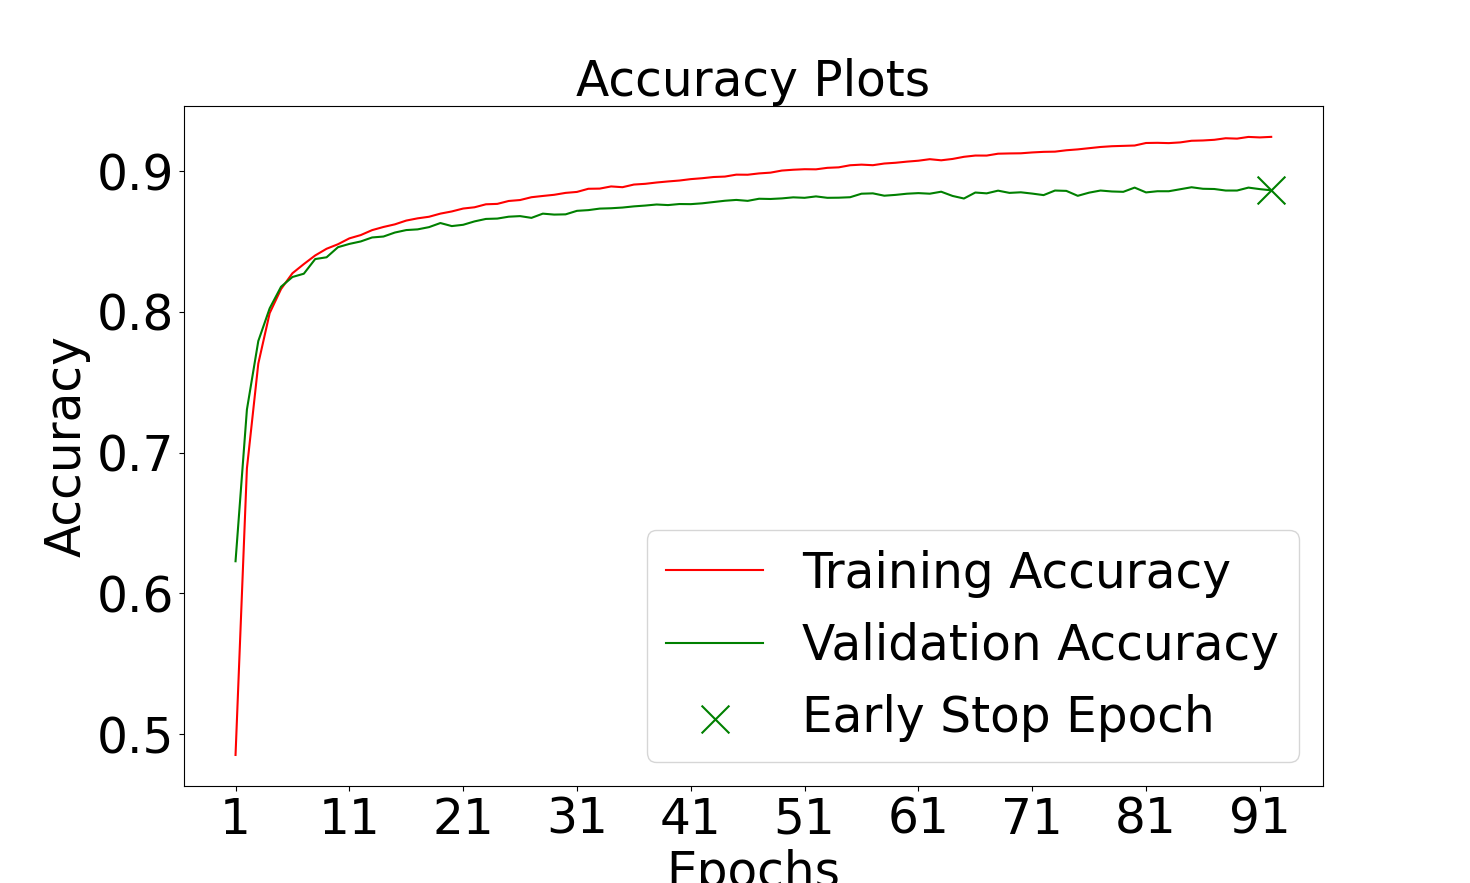
\includegraphics[width=0.45\textwidth]{Figure_mom_acc.png}
        \label{fig:loss_lambda_1e4_2}
    }
    \caption{Loss and Accuracy with Momentum}
    \label{fig:loss_acc_l2}
\end{figure}

\vspace{2cm}

\section{Regularization Experiments}

We added regularization to the backward pass in our neural network model which involved modifying the gradients of the weights during backpropagation. Regularization is necessary to prevent overfitting. The mathematical formulations for adding regularization are as follows - 

L2 Regularization -

\[
\frac{\partial L}{\partial W} = \frac{\partial \text{Loss}}{\partial W} + \lambda W
\]

L1 Regularization -

\[
\frac{\partial L}{\partial W} = \frac{\partial \text{Loss}}{\partial W} + \lambda \cdot \text{sign}(W)
\]

where,\\
$W$, represents the weight\\
$\lambda$, represents the regularization strength

A new config file, \textit{config\_7.yaml} was created. We also increased the number of epochs by \textbf{10\%} and we tested on a range of regularization strengths ranging from 1e-2 to 1e-4 for L2 Regularization, the results were as follows:


\begin{figure}[h!]
    \centering
    \subfigure[Loss]{
        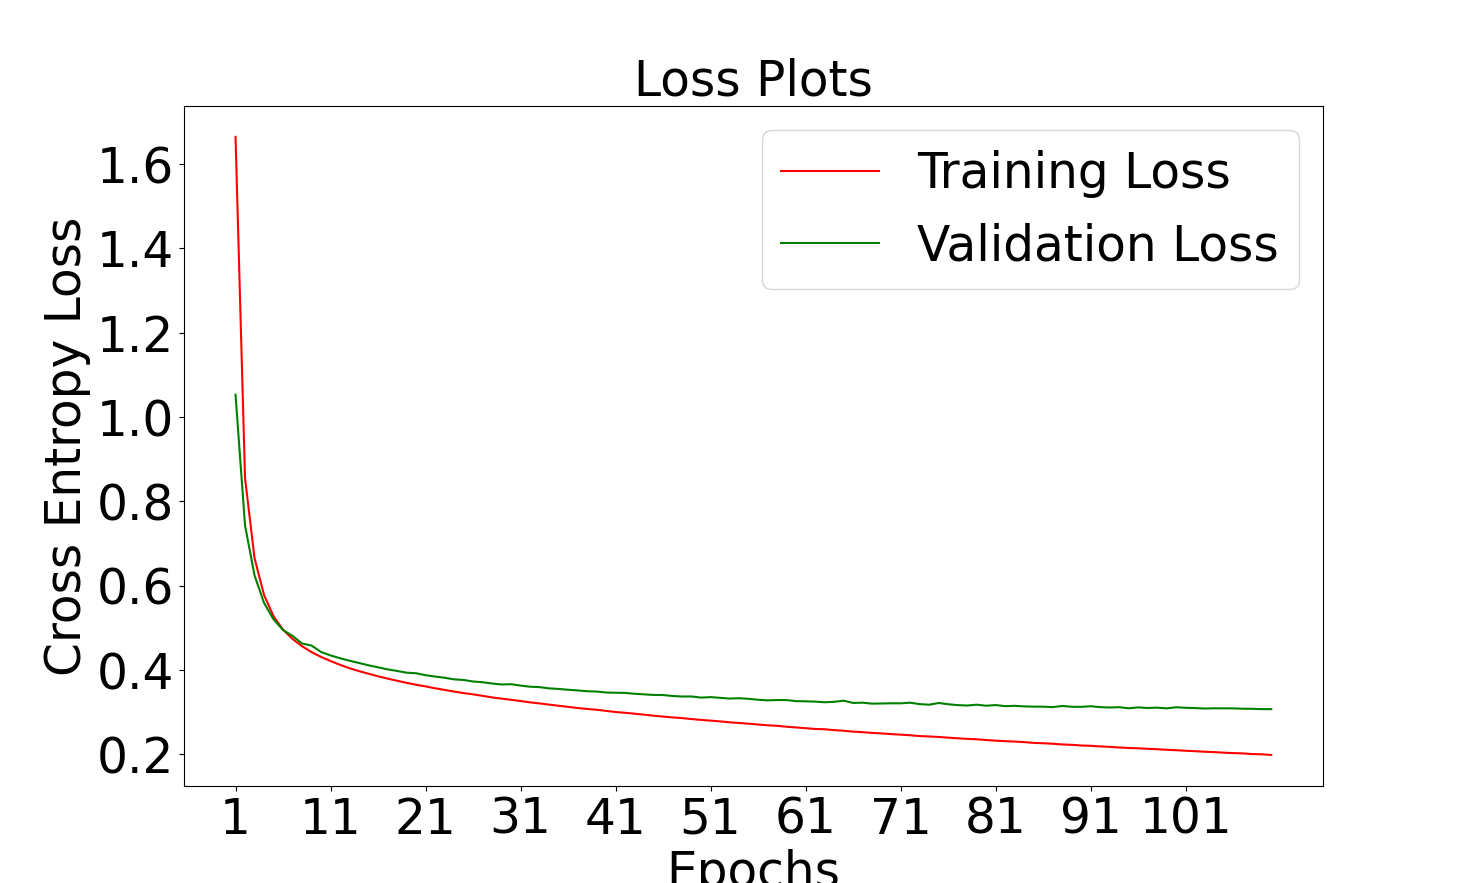
\includegraphics[width=0.45\textwidth]{Figure_reg_e4.png}
        \label{fig:loss_lambda_1e4}
    }
    \hfill
    \subfigure[Accuracy]{
        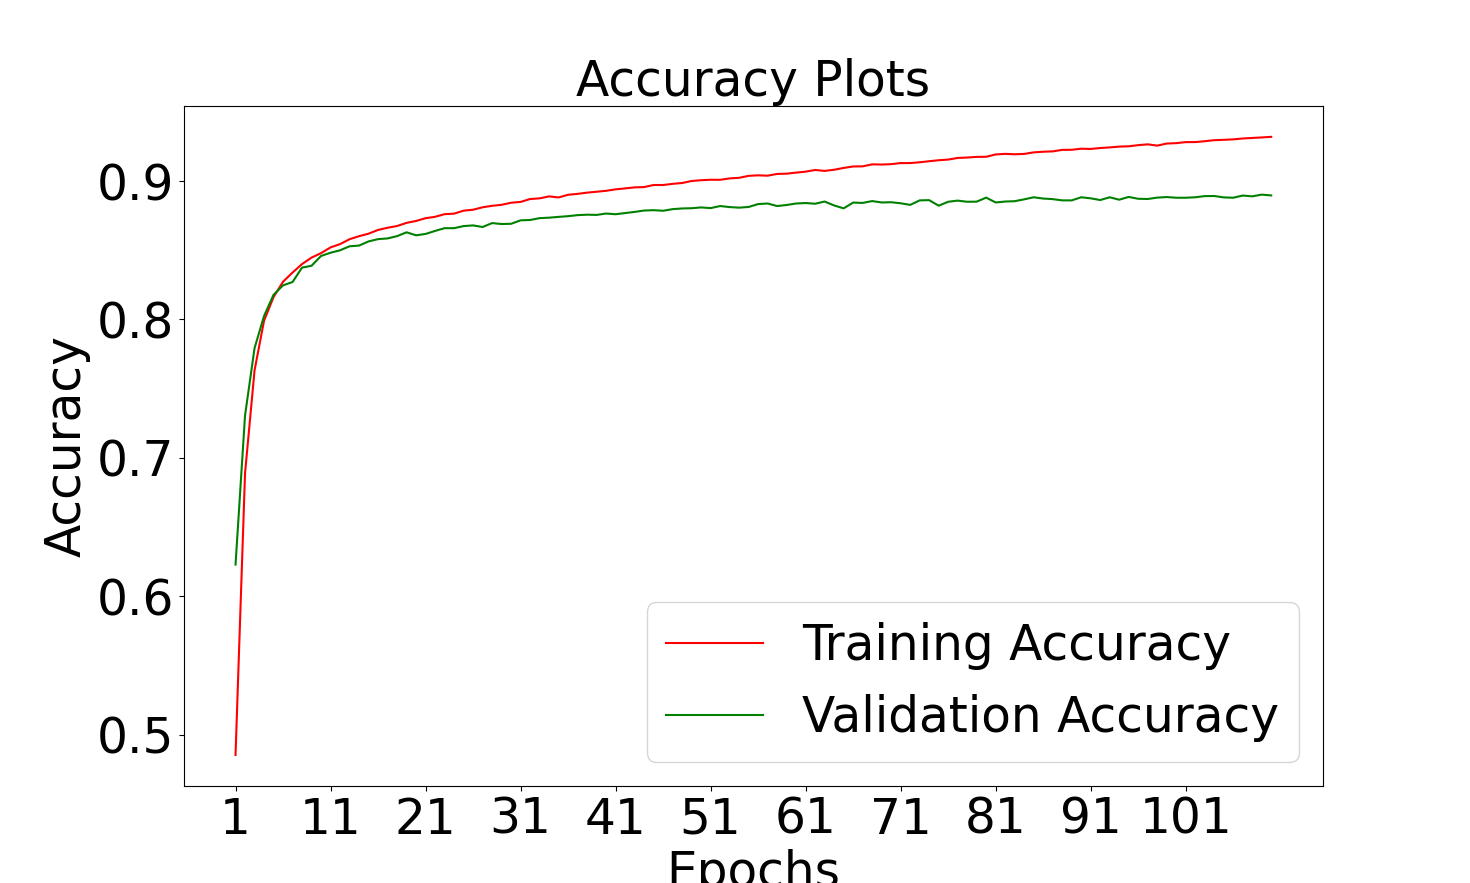
\includegraphics[width=0.45\textwidth]{Figure_reg_acc_e4.png}
        \label{fig:loss_lambda_1e4_2}
    }
    \caption{Loss and Accuracy with L2 regularization (1e-4)}
    \label{fig:loss_acc_l2}
\end{figure}

The best L2 performance on test set (\textbf{88.52\%}) was achieved with $\lambda$ = \textbf{1e-4}. There was an optimal increase in performance as $\lambda$ was decreased.

Similarly, we also tested the network with L1 regularization with values ranging from 1e-3 to 1e-6 and found that the best test accuracy of \textbf{88.53\%} with regularization strength of \textbf{1e-5}. 

\begin{figure}[h!]
    \centering
    \subfigure[Loss]{
        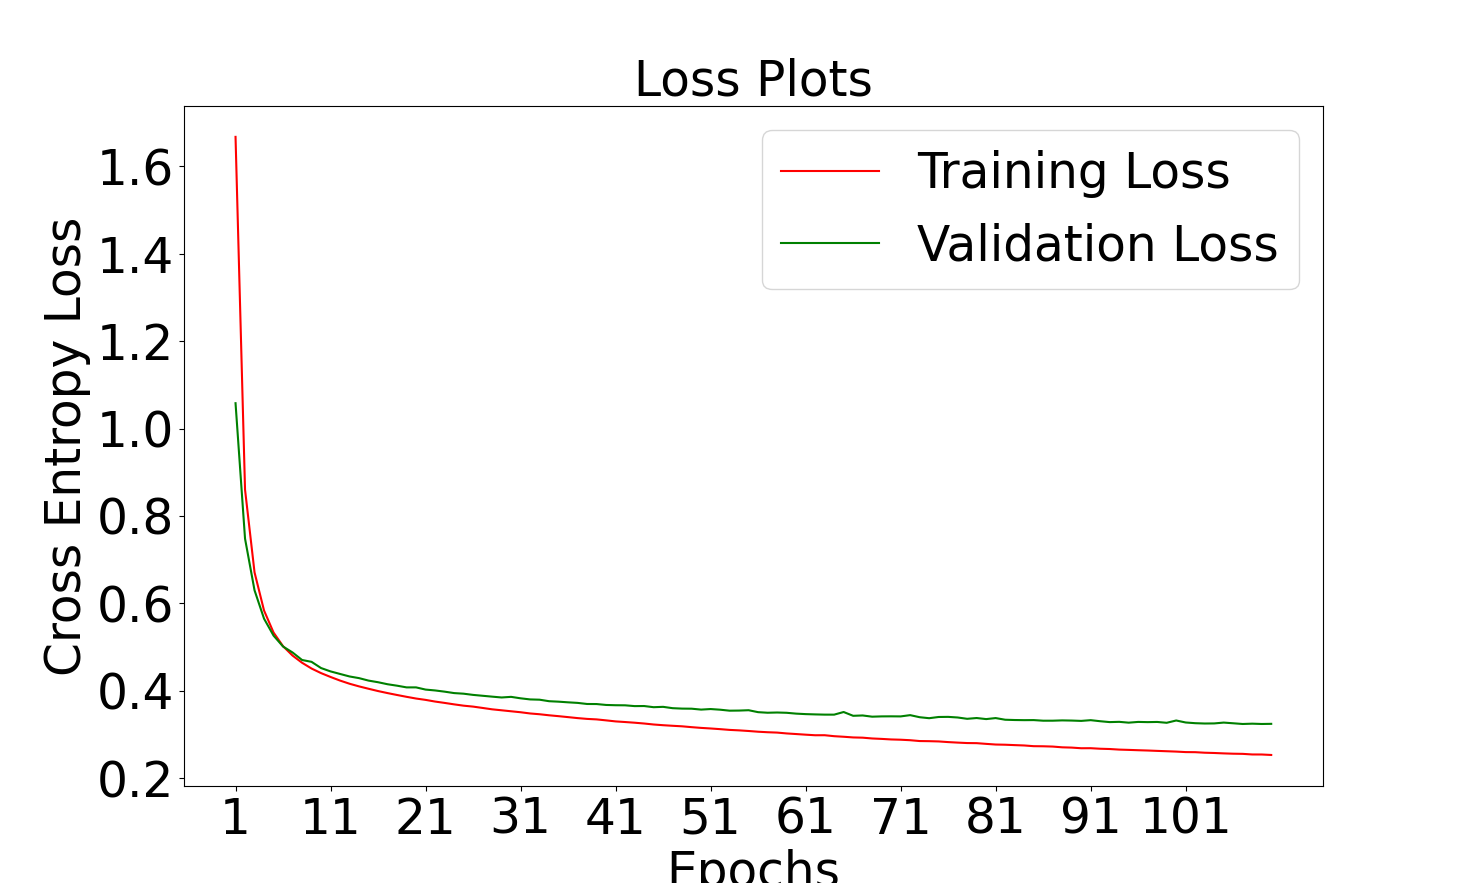
\includegraphics[width=0.45\textwidth]{Figure_l1.png}
        \label{fig:loss_lambda_1e4}
    }
    \hfill
    \subfigure[Accuracy]{
        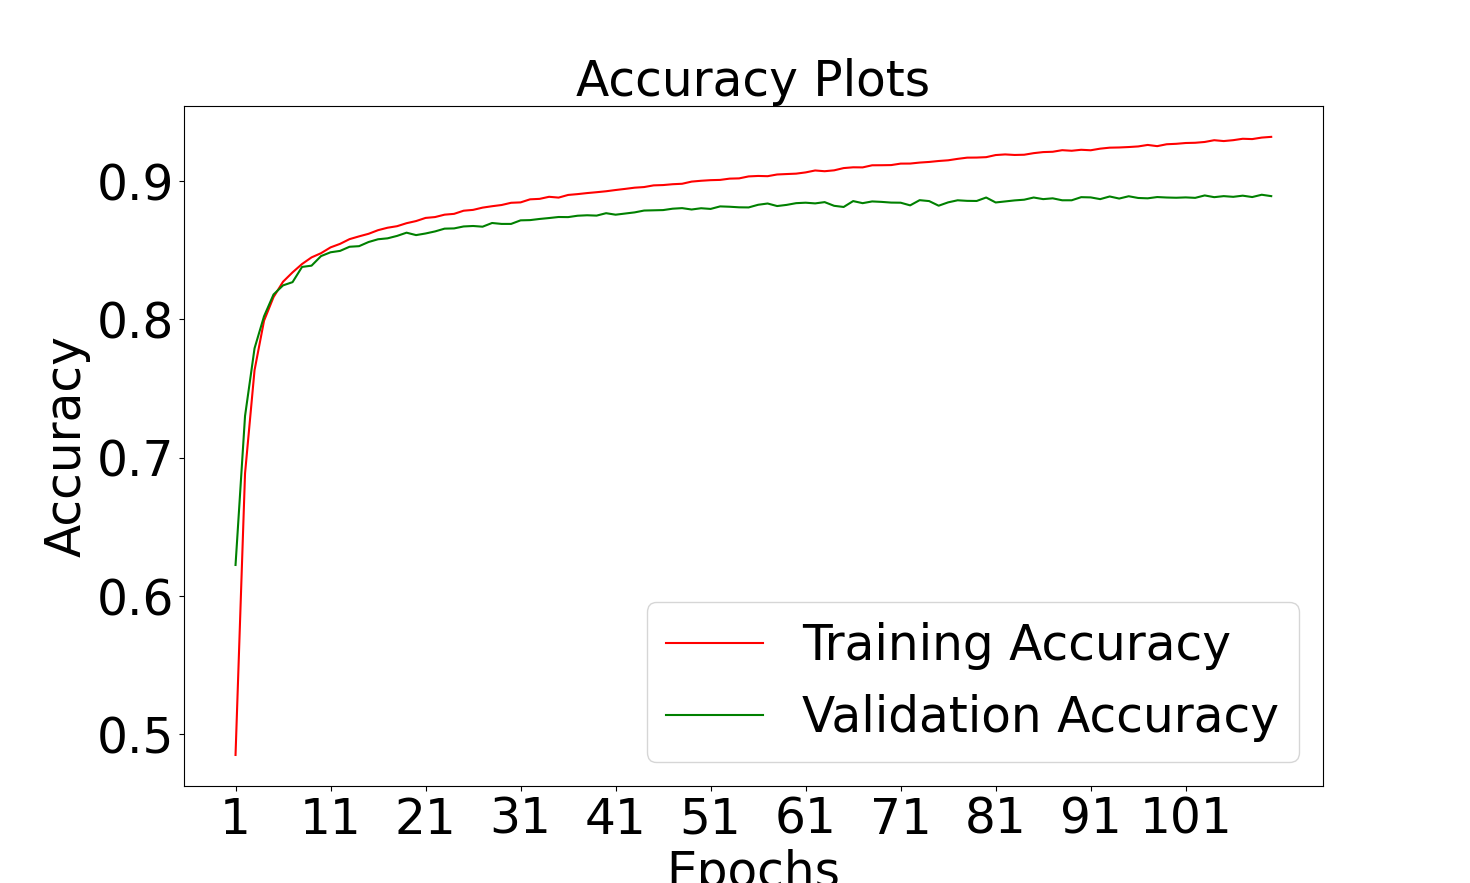
\includegraphics[width=0.45\textwidth]{Figure_l1_e5_acc.png}
        \label{fig:loss_lambda_1e4_2}
    }
    \caption{Loss and Accuracy with L1 regularization (1e-5)}
    \label{fig:loss_acc_l1}
\end{figure}

Overall, L1 regularization showed a higher sensitivity to $\lambda$ values, with larger performance variations. But, similar final test results suggests that both methods were effective at preventing overfitting.


\section{Activation Experiments}

All previous experiments utilized \textbf{ tanh} as the activation function for the hidden layer. So, we tried alternative activation functions such as \textbf{ReLU} and \textbf{sigmoid} -\\

\textbf{Sigmoid}:
$\sigma(x) = \frac{1}{1 + e^{-x}}$\\
\textbf{ReLU}: 
$f(x) = \max(0,x)$\\

A new config file, \textit{config\_8.yaml} was created which included all the hyperperparameters. All the experiments related to the activation functions were performed using that.

We achieved the following results:\\

\subsection{Sigmoid} 
\begin{figure}[h!]
    \centering
    \subfigure[Loss]{
        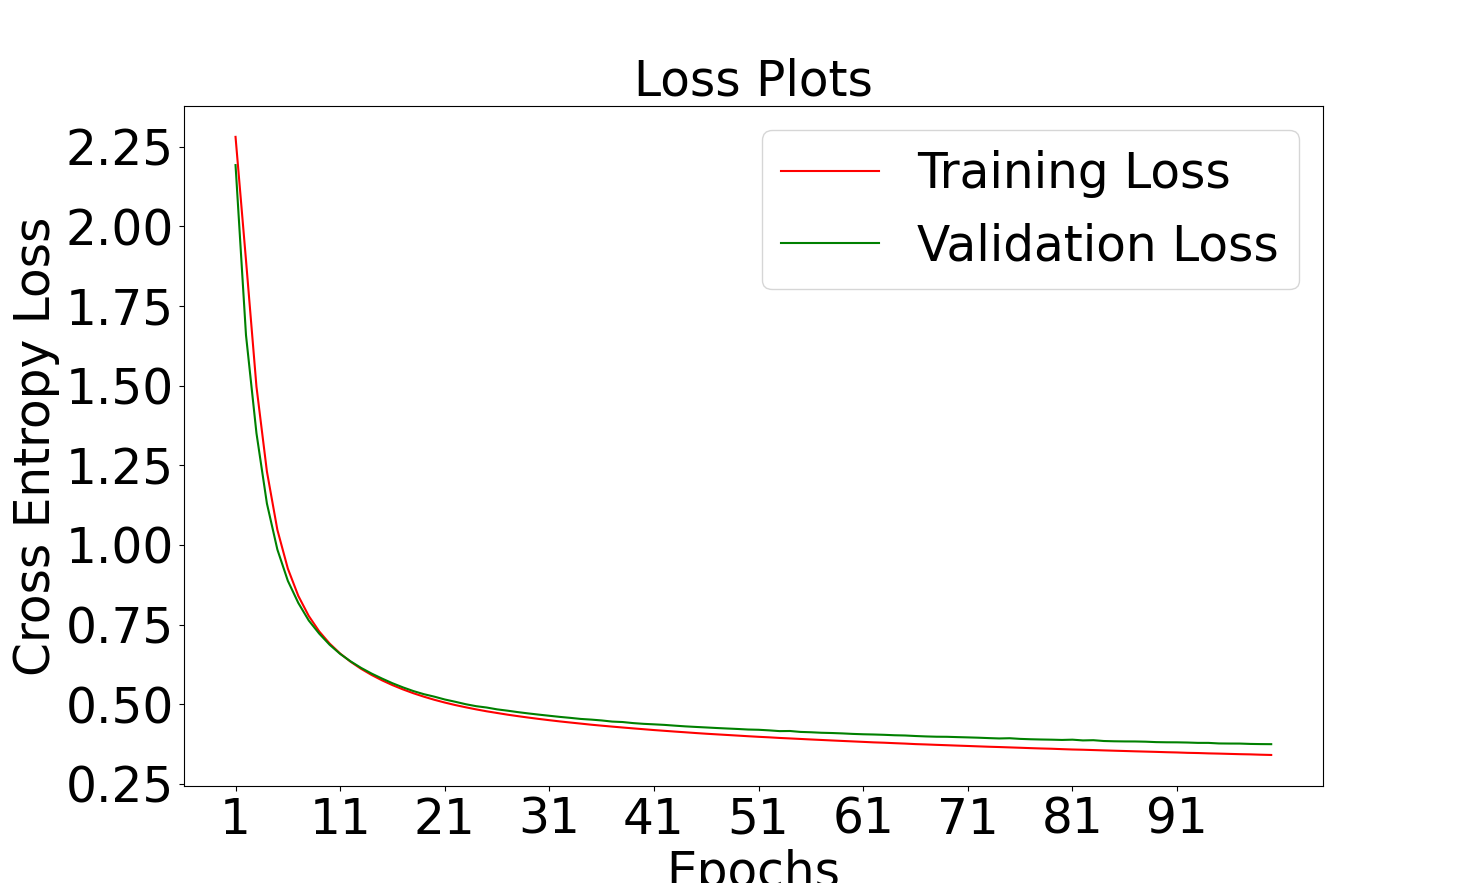
\includegraphics[width=0.45\textwidth]{Figure_sigmoid.png}
        \label{fig:loss_lambda_1e4}
    }
    \hfill
    \subfigure[Accuracy]{
        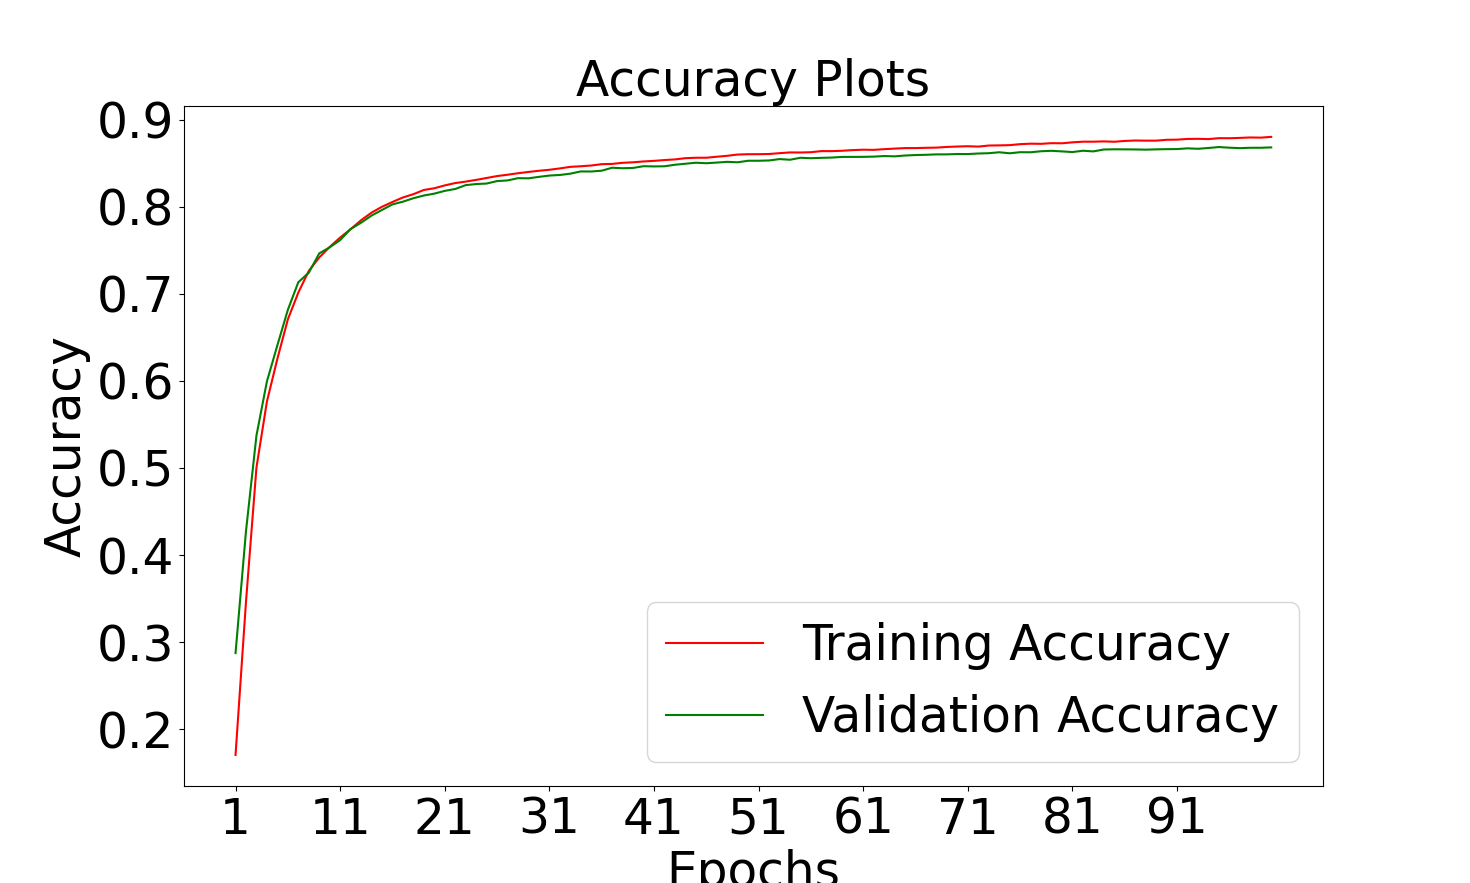
\includegraphics[width=0.45\textwidth]{Figure_sigmoid_acc.png}
        \label{fig:loss_lambda_1e4_2}
    }
    \caption{Loss and Accuracy with Sigmoid function}
    \label{fig:sigmoid}
\end{figure}

Final test accuracy: \textbf{85.83\%}

\subsection{ReLU}

Final test accuracy: \textbf{87.91\%}

According to the results below, Neural Network with ReLU activation function was able to achieve a higher test accuracy than sigmoid. From the graphs in \ref{fig:relu} and \ref{fig:sigmoid}, it can be observed that ReLU was able to converge faster, as evidenced by the steeper initial loss descent. In addition to this, early stopping was triggered for ReLU which suggests better optimization.

\begin{figure}[h!]
    \centering
    \subfigure[Loss]{
        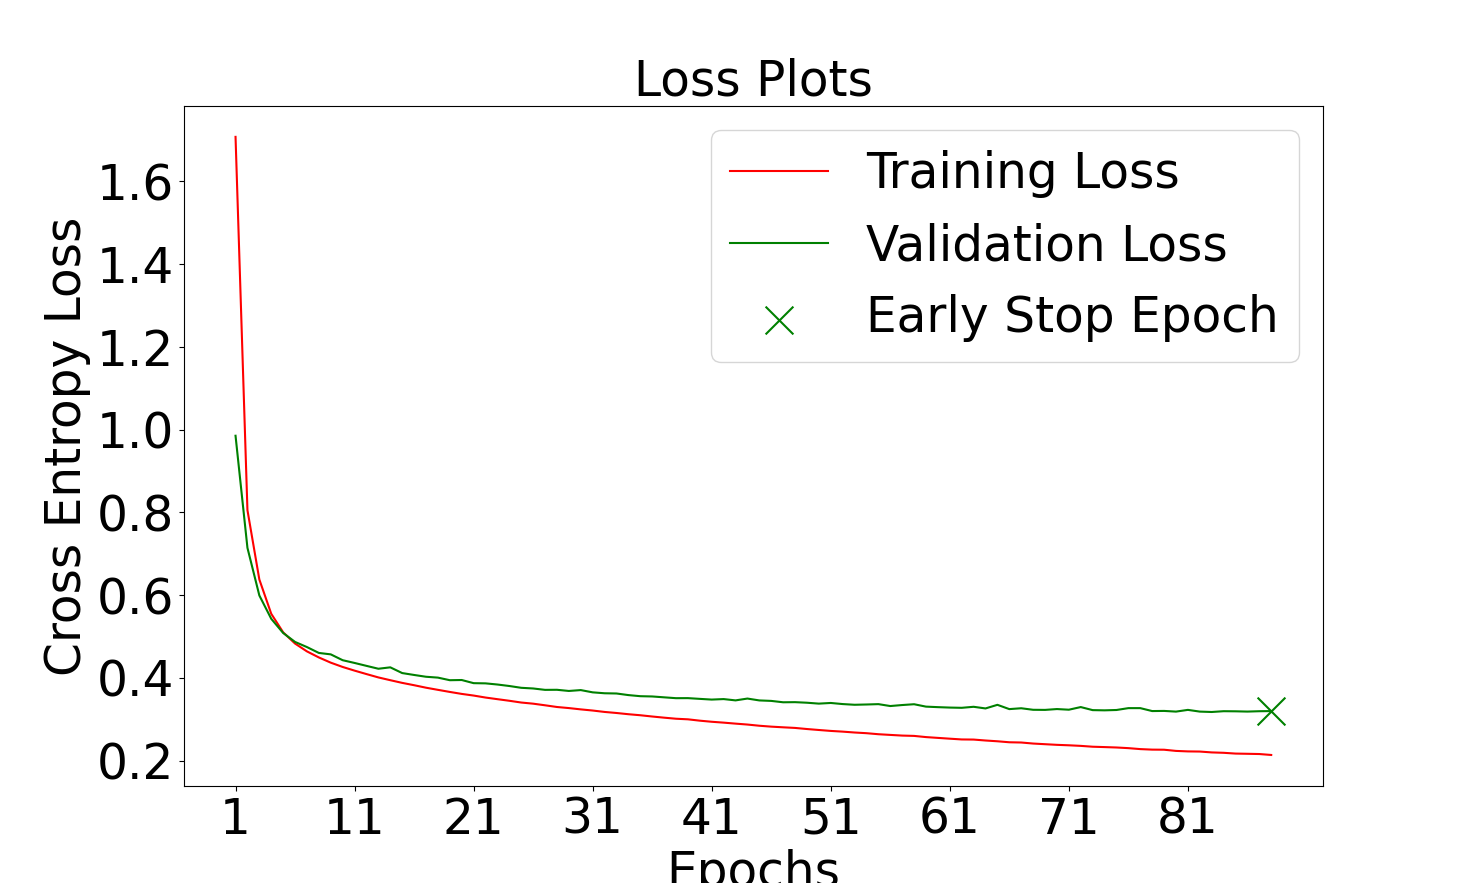
\includegraphics[width=0.45\textwidth]{Figure_relu.png}
        \label{fig:loss_lambda_1e4}
    }
    \hfill
    \subfigure[Accuracy]{
        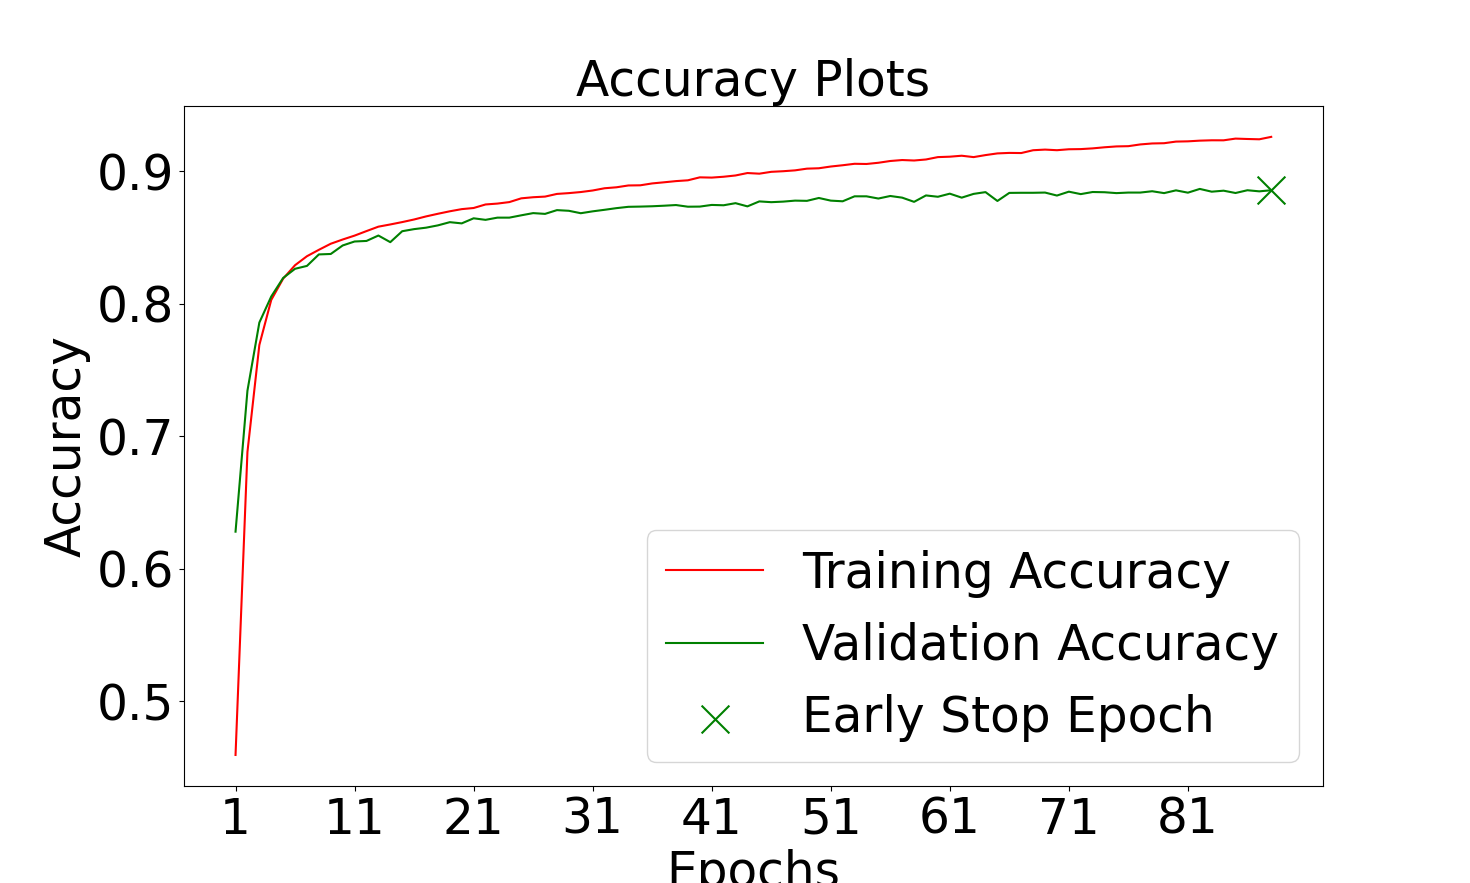
\includegraphics[width=0.45\textwidth]{Figure_relu_acc.png}
        \label{fig:loss_lambda_1e4_2}
    }
    \caption{Loss and Accuracy with ReLU function}
    \label{fig:relu}
\end{figure}
%%%%%%%%%%%%%%%%%%%%%%%%%%%%%%%%%%%%%%%%%%%%%%%%%%%%%%%%%%%%


\end{document}
